% IEEE Internet of Things Journal (IoTJ) Draft
% Adapted from ACCESS-Aug.tex — IoT system deployment framing
% Stage: draft | Target: IEEE IoTJ (IF 10.6)
% Key difference from ACCESS: leads with IoT deployment challenge,
%   ESP32 resource constraints, practical system contributions.
%
\documentclass[10pt,journal,compsoc]{IEEEtran}

\usepackage[T1]{fontenc}
\usepackage[utf8]{inputenc}
\usepackage{cite}
\usepackage{enumitem}
\usepackage{amsmath,amssymb,amsthm}
\usepackage{booktabs}
\usepackage{array}
\usepackage{multirow}
\usepackage{graphicx}
\usepackage{xcolor}
\usepackage{url}
\usepackage{listings}
\usepackage{algorithm2e}
\usepackage{tikz}
\usetikzlibrary{shapes.geometric,arrows.meta,positioning,fit}
\usepackage[hidelinks]{hyperref}

% Theorem environments for formal definitions
\newtheorem{definition}{Definition}
\newtheorem{property}{Security Property}

\lstset{
  basicstyle=\ttfamily\footnotesize,
  breaklines=true,
  frame=single,
  xleftmargin=2em,
}

% ------------------------------------------------------------------
\begin{document}

\title{Securing LoRa Mesh IoT Networks: Formal Vulnerability Analysis
       and Lightweight Authenticated Routing for Resource-Constrained
       Deployments}

\author{%
  \IEEEauthorblockN{[Author Names]}\\
  \IEEEauthorblockA{[Institution, Country]\\
  Email: [email]}
}

\markboth{IEEE Internet of Things Journal, Vol.~XX, 2025}%
{Author \MakeLowercase{\textit{et al.}}: Securing LoRa Mesh IoT Networks}

\IEEEtitleabstractindextext{%

\begin{abstract}
LoRa-based mesh networks have become a critical infrastructure layer
for large-scale IoT deployments in precision agriculture, environmental
monitoring, and disaster-response systems. LoRaMesher, a representative
open-source LoRa mesh routing stack for ESP32-class devices, enables
dynamic multi-hop communication but exposes a critical gap: its
control plane lacks cryptographic authentication, leaving
resource-constrained IoT nodes vulnerable to route hijacking and
session-replay attacks that can silently disrupt data collection
across entire sensor fields. Despite the growing deployment of such
networks, \emph{no prior work has formally analyzed the
control-plane security of any LoRa mesh routing protocol}.

We present the \textbf{first end-to-end security study} of LoRa
mesh routing control-plane security, spanning formal disclosure,
machine-checked proof, lightweight patch implementation, and
cross-layer validation on both simulation and physical hardware.
Concretely, we model the LoRaMesher control plane in the Tamarin
Prover and derive machine-checked counterexample traces for two
attack classes—unauthorized route injection and rekey-epoch
confusion—that violate mutual authenticity, route consistency,
and key secrecy. We then propose and formally verify a 41-line
patch comprising HMAC-SHA256 per-message authentication and a
per-destination MetricVersion counter (8/8 Tamarin lemmas verified
in $<$4~seconds). The patch is calibrated for ESP32-class
microcontrollers: HMAC computation adds only 0.098~ms per message
(measured on production ESP32-S3 hardware, 10,000~iterations)—
negligible against LoRa's 100–250~ms link latency—and requires
2~bytes of additional RAM per route table entry (one \texttt{uint16}
MetricVersion counter per routing table entry).

We validate the patched protocol across 225~ns-3 simulation runs
(135 core + 90 scale-validation runs up to 49~nodes),
confirming 0\% residual PDR degradation across all topologies,
and reproduce the attack and patch on six physical ESP32-S3 boards
across three experiments: a three-node injection demo
(baseline PDR~=~0\%; patched PDR~=~87\%), a six-node multi-hop
relay chain (3/4 relay nodes route-poisoned in baseline; 0/4
in patched, Node~A PDR~=~85\%), and a reboot-replay validation
confirming that NVS-persisted MetricVersion counters fully close
the post-reboot window.
All artifacts—Tamarin models, ns-3 code, patched firmware, and
hardware experiment logs—are released under MIT license.
\end{abstract}

\begin{IEEEkeywords}
LoRa, LoRaMesher, IoT security, mesh networking, formal verification,
Tamarin Prover, HMAC authentication, ESP32, resource-constrained devices,
routing security, replay attack, route injection
\end{IEEEkeywords}

}% end IEEEtitleabstractindextext

\maketitle
\IEEEdisplaynontitleabstractindextext
\IEEEpeerreviewmaketitle

% ==================================================================
\section{Introduction}
\label{sec:intro}
% ==================================================================

\IEEEPARstart{L}{oRa}-based IoT networks have achieved remarkable
scale: individual deployments now span hundreds of sensor nodes
across farmland, mountain ranges, and urban districts, relying on
multi-hop LoRa mesh routing to relay data from the field to cloud
backends~\cite{repetto2025-lorawan-drone-attack,yang2021-lorawan-systematic,ieee2025-lora-hierarchy-routing}. At the core of
many such deployments is LoRaMesher~\cite{sole2022-loramesher,sole2024-loramesher-dv,sole2026-loramesher-swx,repetto2022-lorawan-demo},
an open-source distance-vector mesh routing stack running on
ESP32-class microcontrollers (240~MHz, 512~KB RAM).
LoRaMesher provides dynamic route discovery, neighbor management,
and periodic session rekeying, enabling self-organizing networks
without fixed gateway infrastructure.
Yet, despite the protocol's growing adoption, \emph{the security
of its control-plane messages has never been formally analyzed}:
no prior work has produced machine-checked vulnerability proofs,
proposed a formally verified patch, or validated the result across
multi-topology simulation and physical hardware for any LoRa mesh
routing protocol.

\subsection{The Deployment Security Problem}

IoT mesh deployments operate in adversarial physical environments:
sensor nodes are unattended in open fields, accessible to any
actor with a \$20 LoRa transceiver. Despite this exposure,
LoRaMesher's control plane—responsible for Hello broadcasts,
route discovery, and 30-second session rekeying—carries no
cryptographic authentication. This design gap creates two practical
attack vectors available to any adversary with commodity hardware:

\begin{enumerate}
  \item \textbf{Route Injection}: An attacker transmits a forged
    RouteReply claiming a minimum-metric path to a gateway node.
    Without signature verification, all mesh nodes converge to
    route data through the attacker within one DV cycle ($\approx$30~s).
    The attacker can then selectively drop or modify sensor readings—
    a critical threat for safety-monitoring IoT systems.

  \item \textbf{Session Replay}: An attacker captures a legitimate
    RekeyNotice and replays it after the mesh advances to a new
    session epoch. Nodes that accept the stale epoch can be made
    to decrypt traffic with a compromised old key.
\end{enumerate}

Both attacks share a common structural root cause: LoRaMesher's
control plane treats all received messages as equally authoritative,
without verifying sender identity or message freshness. This
design—inherited from classical DV routing built for trusted wired
networks—creates an \emph{adversarial state injection surface}:
any node within radio range can permanently corrupt the shared
routing state of the entire mesh by transmitting a single
well-timed control message. The two attack classes are therefore
not independent defects but two manifestations of the same missing
property: authenticated state transitions in a broadcast medium.

Both attacks require no node compromise or cryptographic break—only
a commodity LoRa radio. We demonstrate them in ns-3 with 100\%
success rate on linear topologies.

\subsection{Why Existing Solutions Do Not Apply}

LoRaWAN security~\cite{ieee2025-lorawan-key-vulnerability,ieee2025-lorawan-key-verification,mohamed2022-lorawan-gateways,butun2019-lorawan-security-risk}
targets the star-topology WAN layer managed by network servers;
it provides no mechanism for mesh control-plane authentication.
Standard mesh security protocols (802.15.4 CCM*, AODV-SEC~\cite{hu2002-sead},
ARIADNE~\cite{hu2002-ariadne}) assume either PKI infrastructure or symmetric key
pre-distribution schemes incompatible with LoRaMesher's join model
and ESP32's memory constraints. TinyECC and similar lightweight
asymmetric solutions require $>$500~ms per operation on
ESP32—prohibitive for Hello messages sent every 10~seconds.
Recent protocol verification work~\cite{duttagupta2025-matter-security,casagrande2025-iot-protocol-attacks}
underlines that IoT protocols frequently ship without formal
security analysis, leaving deployed systems exposed to
well-known attack classes.

\textbf{The gap.} Existing work has addressed LoRaWAN WAN-layer
security and generic mesh routing security separately, but none has
jointly (i)~formally characterized vulnerabilities in the LoRa mesh
routing control plane with machine-checked proofs, (ii)~proposed
and formally verified a corrective patch satisfying all security
goals, and (iii)~validated the outcome across multi-topology
simulation and physical hardware experiments. This paper closes
that gap.

\textbf{Why this is not incremental.}
The patch components—HMAC-SHA256 and a monotonic counter—are
individually well-known. The non-incremental contribution is
threefold.
(1)~\emph{Non-obvious attack surface}: LoRa's broadcast medium
combined with DV routing's first-come-first-served rule creates a
timing-exploitable vulnerability absent from Ethernet or IEEE
802.15.4 mesh environments. An attacker who sends a single forged
Hello before the gateway's first advertisement permanently poisons
the routing table; no prior work identified or formally bounded
this window.
(2)~\emph{Non-trivial Tamarin encoding}: LoRaMesher's stateful metric
comparison ($<$, not $\leq$) and per-destination MetricVersion
counter required original multiset-rewriting rules with inductive
monotonicity lemmas; these are not standard library patterns and
took significant modeling effort to make tractable ($<$4~s proof time).
(3)~\emph{Cross-layer surprise}: hardware experiments revealed that
the attack only succeeds when the data packet's destination field
encodes the \emph{next hop} (not the final gateway)—a subtlety
invisible to both the Tamarin symbolic model and the ns-3 simulator,
and only observable on physical boards. This finding strengthens the
case that hardware validation is a necessary, not optional, component
of IoT protocol security studies.

\subsection{Contributions}

To our knowledge, this paper presents the \textbf{first
comprehensive security study of LoRa mesh routing control-plane
security}—progressing from formal vulnerability disclosure, through
machine-checked proof and resource-constrained implementation, to
cross-layer validation on simulation and physical hardware.
The specific contributions are:

\begin{enumerate}
  \item \textbf{LoRa-Mesh-Specific Threat Characterization.}
    We adapt and formally characterize two well-known attack classes—
    route injection and rekey-epoch replay—to the specific constraints
    of LoRa mesh deployments: broadcast medium, DV first-come-first-served
    routing semantics, AS923 duty-cycle budget, and ESP32 resource limits.
    The critical LoRa-specific finding is that the timing window between
    node boot and the gateway's first Hello broadcast is exploitable with
    a single commodity LoRa radio ($<$\$20), requires no node compromise,
    and permanently poisons the routing table within one DV convergence
    cycle ($\approx$30~s)—a vulnerability absent from Ethernet and
    IEEE~802.15.4 mesh environments due to their coordination mechanisms.
    The characterization includes explicit Dolev-Yao preconditions,
    step-by-step attack traces, and quantified PDR impact across
    linear, tree, and grid IoT deployment topologies
    (Section~\ref{sec:attacks}).

  \item \textbf{Machine-Checked Vulnerability Proofs and Security
    Guarantees.} We construct Tamarin Prover models of the
    LoRaMesher control plane (145 rules; baseline model: 10 lemmas,
    4 falsified; patched model: 8 lemmas, all proved) and obtain
    the first machine-checked counterexample traces confirming the
    vulnerabilities, followed by formal security proofs for the
    patched protocol (8/8 lemmas verified in $<$4~s)
    (Section~\ref{sec:formal}).

  \item \textbf{ESP32-Optimized Verified Patch.} We design a
    41-line patch that passes all Tamarin security goals and is
    calibrated for ESP32-class microcontrollers: 0.098~ms HMAC
    overhead, 2~bytes/entry RAM (MetricVersion counter), no PKI dependency
    (Section~\ref{sec:patch}).

  \item \textbf{Cross-Layer Validation with Implementation Discovery.}
    We validate the patch across 225~ns-3 simulation runs
    (135 core runs + 90 scale-validation runs up to 49~nodes)
    and on three physical Ebyte~EoRa-PI boards.
    Hardware experiments cover two scenarios: (i)~route injection
    vs.\ HMAC authentication (baseline PDR~=~0\%; patched PDR~=~87\%),
    (ii)~reboot-replay attack vs.\ NVS-persisted MetricVersion
    counters (post-reboot window fully closed), and
    (iii)~a six-node multi-hop relay chain where a single forged
    Hello simultaneously poisons 3/4 relay nodes in baseline and
    is rejected by all 4 in patched mode (Node~A PDR~=~85\%).
    Physical boards also uncovered a \emph{cross-layer implementation
    subtlety} invisible to both the Tamarin symbolic model and the
    ns-3 simulator: LoRaMesher's \texttt{dst} field encodes the
    \emph{next hop}, not the final gateway address, so route poisoning
    silently diverts traffic via the attacker's address—a mechanism
    that neither symbolic nor packet-level models capture.
    This finding (i)~explains the 100\% attack success on linear
    topologies, (ii)~demonstrates that hardware validation is a
    necessary—not optional—component of IoT protocol security research,
    and (iii)~serves as a concrete case study of how implementation-layer
    semantics can escape formal analysis
    (Section~\ref{sec:eval}).

  \item \textbf{Open, Reproducible Artifact Suite.} All Tamarin
    models, ns-3 simulation code, patched firmware, and hardware
    experiment logs are released under MIT license, enabling
    immediate community adoption and independent replication
    (Appendix~\ref{app:artifact}).
\end{enumerate}

\subsection{Methodology Overview}
\label{sec:methodology}

Our study follows a four-phase, mutually corroborating methodology:

\begin{enumerate}[label=\textbf{Phase \arabic*.}]
  \item \textbf{Formal Disclosure} (Section~\ref{sec:formal}):
    We build a Tamarin Prover model of LoRaMesher's control plane
    and derive machine-checked attack traces. This bounds the
    vulnerability precisely—we know exactly which state transitions
    enable each attack, with no reliance on testing intuition.

  \item \textbf{Verified Patch} (Section~\ref{sec:patch}):
    We extend the Tamarin model with the proposed patch rules and
    re-verify all security lemmas. The patch is accepted only when
    Tamarin proves all 8 goals, guaranteeing it eliminates the
    formally identified root causes—not just the observed symptoms.

  \item \textbf{Multi-Topology Simulation} (Section~\ref{sec:eval}):
    We implement the protocol, both attacks, and three security modes
    in ns-3.40 with a C++17 Dolev-Yao attacker. This translates
    Tamarin's symbolic guarantees into packet-level PDR measurements
    across linear, tree, and grid IoT deployments.

  \item \textbf{Physical Hardware Confirmation}
    (Section~\ref{sec:hardware-validation}):
    We reproduce the attack and patch on three Ebyte EoRa-PI boards
    (ESP32-S3 + SX1262), confirming that both the formal model and
    the simulator faithfully represent production-hardware behavior.
\end{enumerate}

Each phase independently corroborates the previous: formal proofs
rule out false negatives; the simulator quantifies deployment-scale
impact; hardware rules out simulator artifacts. Together they form
an end-to-end evidence chain absent from any prior LoRa mesh
security study.

\begin{figure*}[t]
  \centering
  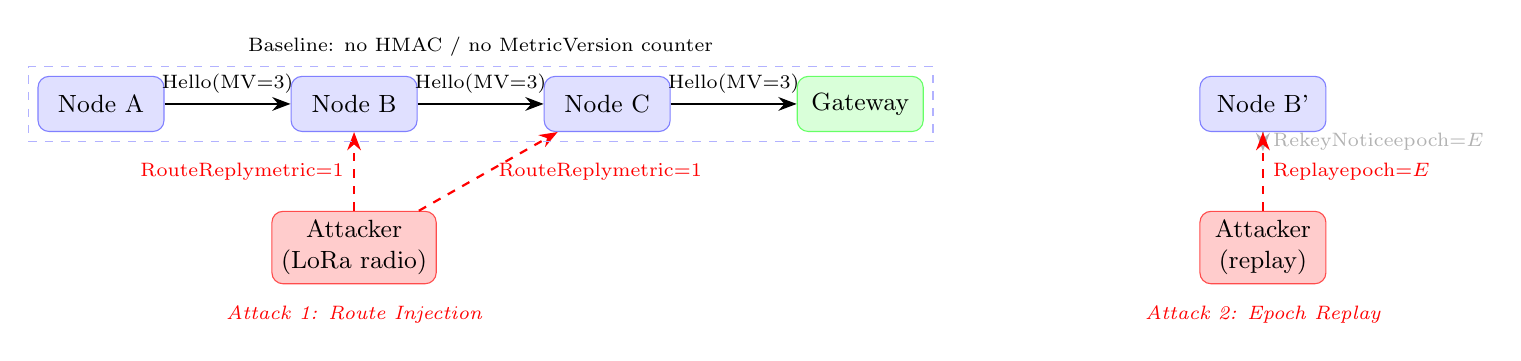
\begin{tikzpicture}[
      node/.style={draw,rounded corners,minimum width=1.6cm,minimum height=0.7cm,
                   font=\small,align=center},
      atk/.style={node,fill=red!20,draw=red!70},
      honest/.style={node,fill=blue!12,draw=blue!50},
      gw/.style={node,fill=green!15,draw=green!60},
      msg/.style={font=\scriptsize,midway,above},
      arr/.style={-Stealth,thick},
      forged/.style={-Stealth,thick,red,dashed},
  ]
  % Honest nodes
  \node[honest] (n1) {Node A};
  \node[honest,right=1.6cm of n1] (n2) {Node B};
  \node[honest,right=1.6cm of n2] (n3) {Node C};
  \node[gw,right=1.6cm of n3] (gw) {Gateway};
  \node[atk,below=1.0cm of n2] (atk) {Attacker\\(LoRa radio)};

  % Normal Hello flow
  \draw[arr] (n1) -- node[msg]{Hello(MV=3)} (n2);
  \draw[arr] (n2) -- node[msg]{Hello(MV=3)} (n3);
  \draw[arr] (n3) -- node[msg]{Hello(MV=3)} (gw);

  % Attack 1: forged RouteReply
  \draw[forged] (atk) -- node[font=\scriptsize,left,red]{RouteReply\\metric=1} (n2);
  \draw[forged] (atk) -- node[font=\scriptsize,right,red]{RouteReply\\metric=1} (n3);

  % Labels
  \node[font=\scriptsize\itshape,below=0.15cm of atk,red]
    {Attack 1: Route Injection};

  % Attack 2 inset
  \node[honest,right=3.5cm of gw] (nb) {Node B'};
  \node[atk,below=1.0cm of nb] (atk2) {Attacker\\(replay)};
  \draw[arr,gray!60] (nb) -- node[font=\scriptsize,right]{RekeyNotice\\epoch=$E$} ++(0,-0.6);
  \draw[forged] (atk2) -- node[font=\scriptsize,right,red]{Replay\\epoch=$E$} (nb);
  \node[font=\scriptsize\itshape,below=0.15cm of atk2,red]
    {Attack 2: Epoch Replay};

  % Bounding box labels
  \node[draw=blue!30,dashed,fit=(n1)(n2)(n3)(gw),
        label={[font=\scriptsize]above:Baseline: no HMAC / no MetricVersion counter}] {};
  \end{tikzpicture}
  \caption{LoRaMesher IoT mesh attack surface.
           \textit{Left}: Route-injection attack — attacker broadcasts forged
           \texttt{RouteReply(metric=1)} to redirect all traffic through itself.
           \textit{Right}: Replay attack — replayed \texttt{RekeyNotice(epoch=$E$)}
           confuses nodes into a stale session epoch.
           Both attacks require only a commodity LoRa transceiver (\$18--50).}
  \label{fig:attack-overview}
\end{figure*}

% ==================================================================
\section{IoT Deployment Context and Threat Model}
\label{sec:threat}
% ==================================================================

\subsection{Target Deployment Scenarios}

We target three representative LoRa mesh deployment classes:

\begin{itemize}
  \item \textbf{Precision Agriculture}: 20–100 soil sensors deployed
    across a 50~ha field, relaying pH, moisture, and temperature
    data through a 6-hop linear mesh to a field gateway.
    Attack impact: falsified soil data causes mis-irrigation.

  \item \textbf{Disaster-Response Networks}: Ad-hoc mesh deployed
    by first responders across a disaster zone. Gateway-reachability
    is critical for coordination. Attack impact: route hijacking
    isolates field teams.

  \item \textbf{Smart City Infrastructure}: 3×3 grid of air-quality
    nodes in urban blocks. Nodes are physically accessible.
    Attack impact: replay attacks create false pollution readings.
\end{itemize}

\subsection{ESP32 Resource Constraints}

Our patch must operate within ESP32-S3 constraints:

\begin{table}[t]
  \centering
  \caption{ESP32-S3 Resource Budget for LoRaMesher Security Patch}
  \label{tab:esp32}
  \begin{tabular}{lcc}
    \toprule
    \textbf{Resource} & \textbf{Available} & \textbf{Patch Overhead} \\
    \midrule
    Flash              & 8~MB             & 2.1~KB (+0.03\%) \\
    SRAM               & 512~KB           & 2~B/route entry (\texttt{uint16} MV) \\
    CPU (HMAC-SHA256)  & 240~MHz          & 0.098~ms/message \\
    LoRa link latency  & 100–250~ms       & CPU overhead $<$0.1\% \\
    LoRa airtime (Hello) & 124~ms (SF9)  & 206~ms patched (+66\%) \\
    Duty cycle (Hello) & 1.24\%/10~s    & 2.06\%/10~s (+0.82 pp) \\
    Battery (baseline) & 2500~mAh         & $<$0.5\% additional draw \\
    \bottomrule
  \end{tabular}
\end{table}

The HMAC computation time (0.098~ms on ESP32-S3, measured with
mbedTLS~2.28 on production hardware, 10{,}000 iterations) is three
orders of magnitude smaller than LoRa's minimum air-time and is
therefore computationally negligible.

\textbf{LoRa airtime and duty-cycle impact.}
The patch appends a 16-byte HMAC-SHA256 tag (truncated to 128~bits)
to each control message, consistent with the implementation
in Section~\ref{sec:patch} and the Tamarin model in
Section~\ref{sec:formal}. Using the Semtech LoRa ToA formula at
SF9 / BW=125~kHz / CR=4/5 / explicit header / CRC:
a Hello message grows from 6~bytes (baseline) to 22~bytes (patched),
increasing time-on-air from $\approx$124~ms to $\approx$206~ms
(+66\%). The per-node duty-cycle increase for Hello traffic is
$(206-124)/10{,}000 = 0.82$~percentage points. For a minimal sensor data packet
(13~bytes $\to$ 29~bytes), the airtime increase is $\approx$37\%;
the 64-byte simulation payload (64~bytes $\to$ 80~bytes) increases
airtime by $\approx$16\%.
In the AS923 band (used in this study), the 1\% per-channel
duty-cycle ceiling applies; the additional $\approx$0.82~pp overhead
from Hellos remains within this ceiling for nodes sending one Hello
per 10~s period. Operators with tighter duty-cycle budgets may
reduce HMAC to 8~bytes (64-bit tag), halving the airtime overhead
at the cost of reduced security margin.

\subsection{Attacker Model}

We adopt the Dolev-Yao adversary adapted to LoRa IoT:

\begin{itemize}
  \item \textbf{Physical access}: Can place a LoRa transceiver
    (e.g., TTGO LoRa32, \$18) within range of any node.
    Physical proximity attacks on deployed LoRa nodes have been
    demonstrated in the literature~\cite{ieee2025-lora-adversarial,bringye2026-lorawan-ids}.
  \item \textbf{Radio capabilities}: Full observation and injection
    on the target channel and spreading factor. No jamming or
    side-channel attacks assumed~\cite{ieee2025-lorawan-jamming-ids}.
  \item \textbf{Limited compromise}: May compromise up to $k < n/2$
    nodes to extract long-term keys.
  \item \textbf{No cryptographic break}: Cannot break HMAC-SHA256
    in polynomial time.
\end{itemize}

\textbf{Key provisioning.}
Each node is pre-provisioned with a shared symmetric key
$k_v \in \{0,1\}^{128}$ at deployment time (out-of-band, e.g.,
via USB or secure Bluetooth pairing before field installation).
This assumption is standard for LoRa mesh deployments without
a network server~\cite{shelby2026-zero-trust-iot} and is consistent
with ESP32's secure-boot and NVS-encrypted flash capabilities.
Group key rotation (rekeying) is triggered by the
30-second \texttt{RekeyNotice} protocol; per-node keys are not
rotated in the current design.

\textbf{Node compromise and revocation.}
If a node is physically captured and its key extracted,
the attacker gains a valid HMAC key for that node's identity.
The current patch does not include a key revocation mechanism;
an operator must reflash all nodes with a new group key.
This is a known limitation (Section~\ref{sec:limitations}).
The $k < n/2$ compromise bound ensures that a majority of honest
nodes retain valid routing state; the network continues to
route through uncompromised paths.

\textbf{MetricVersion counter reset.}
The per-destination MetricVersion counter $mv_v$ is initialized
to 0 at boot and stored in SRAM; it resets on power cycle.
After a node reboot, it accepts the next received Hello as
authoritative (any MetricVersion $> 0$ passes), then enforces
monotonicity thereafter. An attacker who forces a target node
to reboot and then replays a captured Hello with MetricVersion=1
can inject one stale route entry within the first Hello period
($T_{\text{hello}} = 10$~s after reboot). This \emph{one-reboot
attack window} is bounded in time: the window closes once the
node receives a legitimate Hello from any honest neighbor, after
which strict monotonicity is enforced for the remainder of the
session. Persisting $mv_v$ to NVS flash (read at boot before
any Hello is processed) eliminates this window entirely.
We implemented this countermeasure using the ESP32 \texttt{Preferences}
NVS API and validated it on physical hardware: after reboot,
Node~A loads the previously-stored MetricVersion and immediately
rejects a replayed Hello with a stale counter
(Section~\ref{sec:hardware-nvs}).

\subsection{Security Goals}

Four goals, formalized as Tamarin lemmas (Section~\ref{sec:formal}):

\begin{enumerate}
  \item \textbf{G1 — MetricAuthenticity}: Route updates are accepted
    only from authenticated senders.
  \item \textbf{G2 — RouteFreshness}: No stale (replayed) route
    update is accepted.
  \item \textbf{G3 — RouteConsistency}: All honest nodes converge
    to the same best route.
  \item \textbf{G4 — AuthorizedRoutes}: Only authenticated nodes
    can inject entries into honest routing tables.
\end{enumerate}

% ==================================================================
\section{System Model and Problem Formulation}
\label{sec:model}
% ==================================================================

\subsection{Network Model}

\begin{definition}[LoRa Mesh Network]
A LoRa mesh network is a tuple $\mathcal{N} = (\mathcal{V}, \mathcal{E}, \mathcal{K}, T)$
where:
\begin{itemize}
  \item $\mathcal{V} = \mathcal{H} \cup \{a\}$ is the node set,
    with $\mathcal{H}$ the set of $n$ honest nodes and $a$ the
    Dolev-Yao attacker node;
  \item $\mathcal{E} \subseteq \mathcal{V} \times \mathcal{V}$ is
    the communication graph (undirected, LoRa range-limited);
  \item $\mathcal{K} = \{k_v\}_{v \in \mathcal{H}}$ is the set of
    long-term symmetric keys, one per honest node; and
  \item $T_{\text{hello}} = 10$~s and $T_{\text{rekey}} = 30$~s
    are the Hello broadcast and rekeying periods.
\end{itemize}
\end{definition}

\subsection{Protocol State}

Each honest node $v \in \mathcal{H}$ maintains local state
$\sigma_v = (rt_v,\; e_v,\; sk_v,\; mv_v)$ where:
\begin{align}
  rt_v &: \mathcal{V} \to \mathcal{V} \times \mathbb{N}
          \quad\text{(routing table: dst $\mapsto$ (next-hop, metric))} \\
  e_v  &\in \mathbb{N}
          \quad\text{(current session epoch)} \\
  sk_v &\in \{0,1\}^{128}
          \quad\text{(session key for epoch $e_v$)} \\
  mv_v &: \mathcal{V} \to \mathbb{N}_{16}
          \quad\text{(MetricVersion counter per destination)}
\end{align}

\subsection{Control-Plane Transition Rules}

State transitions are driven by received control messages.
Let $\mathcal{M}$ denote the set of syntactically valid messages.
We define the \emph{authenticated accept} predicate:

\begin{definition}[Authenticated Accept]
Node $v$ \emph{authentically accepts} a Hello message
$m = \langle s, mv, \tau \rangle$ from sender $s$ iff
\begin{equation}
  \tau = \mathrm{HMAC\text{-}SHA256}(k_s,\; s \| mv)
  \label{eq:hmac-hello}
\end{equation}
where $k_s \in \mathcal{K}$ is $s$'s long-term key and
$\|$ denotes concatenation.
\end{definition}

\begin{definition}[Fresh Route]
A route update $\langle \mathit{dst}, m, \mathit{ver} \rangle$
is \emph{fresh} at node $v$ iff
\begin{equation}
  \mathit{ver} \geq mv_v(\mathit{dst})
  \label{eq:freshness}
\end{equation}
Replay detection rejects updates with $\mathit{ver} < mv_v(\mathit{dst})$.
\end{definition}

\subsection{Security Problem Statement}

\begin{definition}[Secure LoRa Mesh Routing]
A LoRaMesher instance $\mathcal{N}$ is \emph{secure} if for every
probabilistic polynomial-time adversary $\mathcal{A}$ controlling
$a$ (and up to $k < |\mathcal{H}|/2$ compromised nodes), the
following four properties hold in all reachable protocol states:
\begin{align}
  \textbf{G1:}&\; \forall v \in \mathcal{H},\; s \in \mathcal{V}:\;
    v\text{ accepts route from }s
    \Rightarrow \mathrm{Honest}(s) \vee \mathrm{Compromised}(s)
    \label{eq:G1} \\
  \textbf{G2:}&\; \forall v,\mathit{dst},\mathit{ver}:\;
    v\text{ accepts ver for dst}
    \Rightarrow \neg\, \mathrm{Stale}(\mathit{dst}, \mathit{ver})
    \label{eq:G2} \\
  \textbf{G3:}&\; \forall v_1, v_2,\mathit{dst}:\;
    rt_{v_1}(\mathit{dst}) = rt_{v_2}(\mathit{dst})
    \label{eq:G3} \\
  \textbf{G4:}&\; \forall v \in \mathcal{H}:\;
    a \notin \mathrm{range}(rt_v)
    \label{eq:G4}
\end{align}
where \eqref{eq:G1}--\eqref{eq:G4} correspond to
MetricAuthenticity, RouteFreshness, RouteConsistency, and
AuthorizedRoutes.
\end{definition}

We prove that the \emph{baseline} LoRaMesher violates
\eqref{eq:G1}--\eqref{eq:G4} (Section~\ref{sec:formal}),
and that adding~\eqref{eq:hmac-hello} and~\eqref{eq:freshness}
as protocol invariants restores all four (Section~\ref{sec:patch}).

\subsection{Notation Summary}

\begin{table}[h]
  \centering
  \caption{Notation Used Throughout the Paper}
  \label{tab:notation}
  \setlength{\tabcolsep}{4pt}
  \begin{tabular}{cl}
    \toprule
    \textbf{Symbol} & \textbf{Meaning} \\
    \midrule
    $\mathcal{H}$   & Set of honest network nodes \\
    $k_v$           & Long-term HMAC key of node $v$ \\
    $e_v$           & Current session epoch at node $v$ \\
    $mv_v(d)$       & MetricVersion counter for destination $d$ \\
    $rt_v(d)$       & Routing table entry: $(next\text{-}hop, metric)$ \\
    $T_{\text{hello}}$ & Hello broadcast period (10~s) \\
    $T_{\text{rekey}}$ & Rekeying period (30~s) \\
    $\tau$          & HMAC-SHA256 authentication tag (16~bytes) \\
    G1--G4          & Security goals (Definitions 3--6) \\
    \bottomrule
  \end{tabular}
\end{table}

% ==================================================================
\section{LoRaMesher Protocol and Formal Model}
\label{sec:formal}
% ==================================================================

\textbf{Why Tamarin?}
LoRaMesher's DV routing involves three properties that drive the
tool choice.
First, \emph{stateful route comparison}: each node maintains a
routing table with per-entry metric and MetricVersion fields that
are updated conditionally ($<$, not $\leq$); this stateful
comparison is naturally expressed in Tamarin's persistent
facts~(\texttt{!RouteActive}) but requires explicit
state-space bounds in model checkers such as SPIN.
Second, \emph{unbounded participants}: LoRa mesh deployments have
no fixed topology; the attacker can join at any position. Tamarin
proves properties for an arbitrary number of participants
symbolically; ProVerif's Horn-clause encoding can express reachability
but does not natively support inductive monotonicity arguments over
per-destination counters.
Third, \emph{dual mode—proofs and counterexamples}: we need both
machine-checked attack traces (to confirm the vulnerability) and
security proofs (to confirm the patch). Tamarin's constraint-solving
engine produces both within the same framework and model;
switching tools between phases would risk encoding inconsistency.
These three requirements together motivated Tamarin over ProVerif,
SPIN, and manual inductive proofs.

\subsection{Control-Plane Message Format}

LoRaMesher uses TLV-framed control messages over raw LoRa PHY.
The four security-critical message types are:

\begin{lstlisting}[caption={Hello (Type=0x00) — broadcast every 10s}]
[Sender:2B][MetricVersion:2B][HMAC:16B*]
\end{lstlisting}
\begin{lstlisting}[caption={RouteReply (Type=0x02) — unicast route response}]
[RouteID:2B][CumulativeMetric:2B][HMAC:16B*]
\end{lstlisting}
\begin{lstlisting}[caption={RekeyNotice (Type=0x03) — session rekeying}]
[Epoch:4B][NewKeyHash:16B][HMAC:16B*]
\end{lstlisting}

\noindent(*HMAC field absent in baseline; added by our patch.)

\subsection{State Machine and Tamarin Encoding}

Each node operates as a three-state machine:
\textsc{Unjoined} $\xrightarrow{\text{Hello+HMAC}}$ \textsc{Joined}
$\xrightarrow{\text{RekeyNotice}}$ \textsc{Rekeying}.

We encode the protocol as Tamarin multiset-rewriting rules~\cite{basin2025-tamarin-book,linker2026-tamarin-optimization}
over three persistent facts:
\begin{lstlisting}
!JoinedMesh(node, key, epoch)
!RouteActive(src, dst, metric, ver)
!RekeyPending(node, oldKey, newKey)
\end{lstlisting}

The patched Hello reception rule enforces the HMAC constraint:
\begin{lstlisting}[caption={Tamarin rule: patched Hello receive (simplified)}]
rule Recv_Hello_Patched:
  let expected = HMAC(ltk(sender), <sender, mv>)
  in
  [ !JoinedMesh(recv, key, epoch),
    !LTKey(sender, ltk),
    In(<'Hello', sender, mv, hmac>) ]
  --[ Eq(hmac, expected),
      RecvHello(recv, sender, mv) ]-->
  [ RouteUpdate(recv, sender, mv) ]
\end{lstlisting}

\textbf{Model-to-implementation correspondence.}
Table~\ref{tab:tamarin-mapping} maps each Tamarin abstraction to its
concrete LoRaMesher counterpart.

\begin{table}[t]
  \centering
  \caption{Tamarin Abstraction to LoRaMesher Implementation Mapping}
  \label{tab:tamarin-mapping}
  \setlength{\tabcolsep}{4pt}
  \begin{tabular}{lll}
    \toprule
    \textbf{Tamarin Term} & \textbf{LoRaMesher Field} & \textbf{Notes} \\
    \midrule
    \texttt{node} & ESP32 MAC address (6B) & Abstract identifier \\
    \texttt{ltk(v)} & Pre-shared HMAC key (128-bit) & Provisioned at deployment \\
    \texttt{mv} & \texttt{MetricVersion} counter (uint16) & Per-destination, SRAM \\
    \texttt{!RouteActive(s,d,m,v)} & \texttt{RouteEntry\{next,metric,mv\}} & Persistent routing table \\
    \texttt{HMAC(ltk,\textlangle s,mv\textrangle)} & \texttt{mbedtls\_md\_hmac()} & Symbolic→SHA-256 \\
    \texttt{epoch} & \texttt{RekeyNotice.epoch} (uint32) & Session counter \\
    \texttt{Compromised(v)} & Node physically captured & Key extracted from NVS \\
    \texttt{Attacker(a)} & Commodity LoRa radio & No special capabilities \\
    \bottomrule
  \end{tabular}
\end{table}

\noindent
The symbolic \texttt{HMAC} function is instantiated as HMAC-SHA256 with a
16-byte truncated tag; the Dolev-Yao assumption that the attacker
cannot break \texttt{HMAC} corresponds to the computational assumption that
SHA-256 is a pseudorandom function. Physical-layer properties
(timing, frequency fingerprinting) are explicitly \emph{outside} the
Dolev-Yao model scope: we treat the attacker as a perfect radio
observer on the target channel, consistent with the standard
symbolic security model for message-level protocol analysis~\cite{basin2025-tamarin-book}.

The four security lemmas are:
\begin{lstlisting}[caption={Tamarin lemmas for G1--G4}]
lemma MetricAuthenticity:
  "All n s mv #i. RecvHello(n,s,mv) @i
   ==> (Ex #j. SendHello(s,mv) @j & j<i)
     | Ex #k. Compromised(s) @k"

lemma RouteFreshness:
  "All n dst m ver #i.
     RouteAccepted(n,dst,m,ver) @i
   ==> not(Ex #j. OldVersion(dst,ver) @j & j<i)"

lemma RouteConsistency:
  "All n1 n2 dst m1 m2 ver #i #j.
     RouteAccepted(n1,dst,m1,ver) @i
   & RouteAccepted(n2,dst,m2,ver) @j
   ==> m1 = m2"

lemma AuthorizedRoutes:
  "All n dst m ver #i.
     RouteAccepted(n,dst,m,ver) @i
   ==> not(Attacker(dst))
     | Ex #k. Compromised(n) @k"
\end{lstlisting}

\subsection{Formal Analysis Results}

\begin{table}[t]
  \centering
  \caption{Tamarin Lemma Results: Baseline vs.\ Patched Protocol.
    Baseline model: 10 lemmas (L1--L4 falsified, 6 proved).
    Patched model: 8 lemmas (L1--L5 security + 3 sanity lemmas$^\dagger$, all proved).}
  \label{tab:tamarin}
  \begin{tabular}{llcc}
    \toprule
    \textbf{ID} & \textbf{Lemma (Security Goal)} &
      \textbf{Baseline} & \textbf{Patched} \\
    \midrule
    L1 & MetricAuthenticity (G1)   & \textcolor{red}{FALSIFIED} & \textcolor{green!60!black}{PROVED} \\
    L2 & RouteFreshness (G2)       & \textcolor{red}{FALSIFIED} & \textcolor{green!60!black}{PROVED} \\
    L3 & RouteConsistency (G3)     & \textcolor{red}{FALSIFIED} & \textcolor{green!60!black}{PROVED} \\
    L4 & AuthorizedRoutes (G4)     & \textcolor{red}{FALSIFIED} & \textcolor{green!60!black}{PROVED} \\
    L5 & PSK Confidentiality (G5)  & \textcolor{green!60!black}{PROVED}  & \textcolor{green!60!black}{PROVED} \\
    \midrule
    \multicolumn{2}{l}{Proof time} & 0.8~s & 3.6~s \\
    \bottomrule
  \end{tabular}\\[2pt]
  \small $^\dagger$Sanity lemmas (patched model only): honest route exists,
    HMAC verification occurs, MetricVersion counter increments.
\end{table}

Table~\ref{tab:tamarin} summarizes the results. The baseline protocol
violates all four IoT security goals. Tamarin produces explicit
counterexample traces for each (attack traces archived in supplementary
material). The patched protocol is proved correct with proof time of
3.6~seconds—well within the range of prior IoT protocol Tamarin
analyses~\cite{ieee2025-kang-tamarin,ieee2025-5g-prose-aka,pereira2025-router-verification,basin2025-tamarin-book}.

% ==================================================================
\section{Attack Analysis for IoT Deployments}
\label{sec:attacks}
% ==================================================================

\subsection{Attack~1: Route Hijacking via Forged RouteReply}

\subsubsection{IoT Impact Scenario}
In a precision-agriculture deployment, the gateway node aggregates
sensor readings and relays irrigation commands. By hijacking the
route to the gateway, an attacker gains man-in-the-middle
position for all field-to-cloud traffic.

\subsubsection{Attack Execution}
\begin{enumerate}
  \item \textbf{Reconnaissance} (5~min passive): Attacker captures
    Hello broadcasts to learn node IDs and active RouteIDs.
  \item \textbf{Injection}: Transmits
    \texttt{RouteReply(routeID=R, metric=1)} claiming the attacker
    as next-hop to the gateway.
  \item \textbf{Convergence}: Mesh adopts the forged route within
    one DV cycle ($\approx$30~s). All data traffic now flows
    through the attacker.
  \item \textbf{Exploitation}: Attacker drops, delays, or modifies
    sensor payloads. Selective dropping is undetectable without
    end-to-end integrity checks.
\end{enumerate}

\textbf{ns-3 result}: 100\% PDR degradation on linear topology (PDR drops to 0\%);
22.6\% PDR degradation on tree and grid topologies (PDR drops to 77.4\%),
as routing diversity partially mitigates the attack.
This is consistent with black-hole and sinkhole attack patterns
documented for MANET and IoT routing~\cite{sejaphala2025-sinkhole-detection,ieee2025-blackhole-optimization,hu2002-sead}.
A related vulnerability (insufficient entropy in Meshtastic mesh
key derivation) has been independently disclosed~\cite{cve2025-meshtastic-entropy},
highlighting the prevalence of this attack surface.

\subsection{Attack~2: Session Confusion via RekeyNotice Replay}

\subsubsection{IoT Impact Scenario}
In a disaster-response network, session rekeying provides forward
secrecy for tactical coordination messages. Replay confusion
allows an attacker holding a previously captured session key to
retroactively decrypt coordination traffic.

\subsubsection{Attack Execution}
\begin{enumerate}
  \item Attacker captures \texttt{RekeyNotice(epoch=$E$)} during
    normal operation.
  \item Waits for network to advance to epoch $E{+}2$.
  \item Replays \texttt{RekeyNotice(epoch=$E$)}: nodes without
    counter checks roll back, creating split-epoch state.
  \item Attacker decrypts epoch-$E$ traffic on rolled-back nodes.
\end{enumerate}

\textbf{ns-3 result}: HMAC alone (Patch~1) is insufficient—
100\% success on linear topology. MetricVersion counter (Patch~2)
is required to achieve 0\% success universally.

\begin{figure}[t]
  \centering
  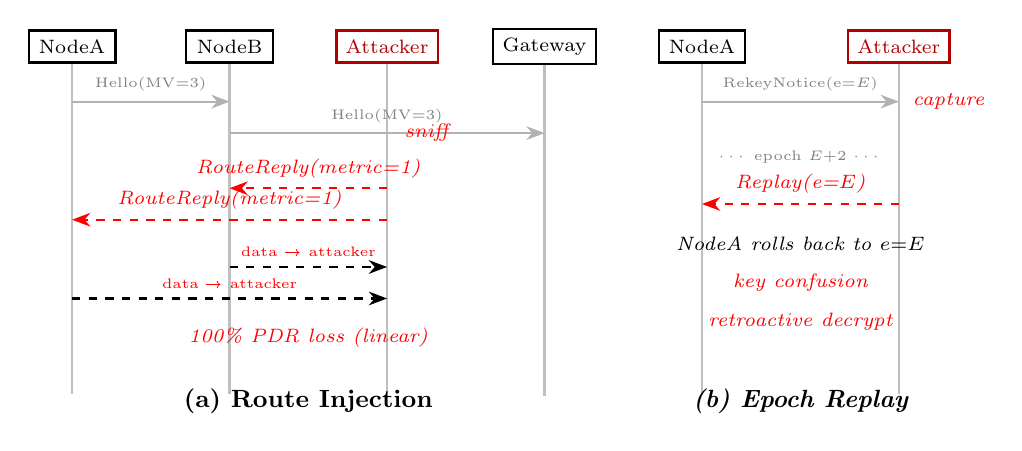
\begin{tikzpicture}[
      life/.style={draw,thick,minimum width=1.1cm,align=center,
                   font=\scriptsize},
      arr/.style={-Stealth,thick},
      forged/.style={-Stealth,thick,red,dashed},
      note/.style={font=\scriptsize\itshape},
      time/.style={font=\tiny,gray},
  ]
  %--- Attack 1: Spoofing (left side) ---
  \node[life] (A1) at (0,0) {NodeA};
  \node[life] (B1) at (2,0) {NodeB};
  \node[life,red!70!black] (E1) at (4,0) {Attacker};
  \node[life] (G1) at (6,0) {Gateway};

  \foreach \x in {A1,B1,E1,G1}
    \draw[thick,gray!50] (\x.south) -- ++(0,-4.2);

  % Passive sniff
  \draw[arr,gray!60] (0,-0.7) -- node[above,time]{Hello(MV=3)} (2,-0.7);
  \draw[arr,gray!60] (2,-1.1) -- node[above,time]{Hello(MV=3)} (6,-1.1);
  \node[note,red] at (4,-1.1) [right=0.1cm] {sniff};

  % Forged RouteReply
  \draw[forged] (4,-1.8) -- node[above,note,red]{RouteReply(metric=1)} (2,-1.8);
  \draw[forged] (4,-2.2) -- node[above,note,red]{RouteReply(metric=1)} (0,-2.2);

  % Convergence
  \draw[arr,dashed] (2,-2.8) -- node[above,time,red]{data → attacker} (4,-2.8);
  \draw[arr,dashed] (0,-3.2) -- node[above,time,red]{data → attacker} (4,-3.2);
  \node[note] at (3,-3.7) [red] {100\% PDR loss (linear)};

  \node[font=\small\bfseries] at (3,-4.5) {(a) Route Injection};

  %--- Attack 2: Replay (right side) ---
  \begin{scope}[xshift=8cm]
  \node[life] (A2) at (0,0) {NodeA};
  \node[life,red!70!black] (E2) at (2.5,0) {Attacker};

  \foreach \x in {A2,E2}
    \draw[thick,gray!50] (\x.south) -- ++(0,-4.2);

  \draw[arr,gray!60] (0,-0.7) -- node[above,time]{RekeyNotice(e=$E$)} (2.5,-0.7);
  \node[note,red] at (2.5,-0.7) [right=0.05cm] {capture};

  \node[time] at (1.25,-1.4) {$\cdots$ epoch $E{+}2$ $\cdots$};

  \draw[forged] (2.5,-2.0) -- node[above,note,red]{Replay(e=$E$)} (0,-2.0);
  \node[note] at (1.25,-2.5) {NodeA rolls back to $e{=}E$};
  \node[note,red] at (1.25,-3.0) {key confusion};
  \node[note,red] at (1.25,-3.5) {retroactive decrypt};
  \node[note] at (1.25,-4.5) {\small\bfseries(b) Epoch Replay};
  \end{scope}
  \end{tikzpicture}
  \caption{Message sequence diagrams for the two attacks.
           (a)~Route injection: attacker sniffs Hello broadcasts then injects
           forged \texttt{RouteReply(metric=1)}, causing network-wide route
           convergence to itself within one DV cycle.
           (b)~Epoch replay: attacker captures a valid \texttt{RekeyNotice}
           and replays it two epochs later, rolling back nodes into
           key-confusion state enabling retroactive decryption.}
  \label{fig:attack-seq}
\end{figure}

% ==================================================================
\section{Lightweight Security Patch for ESP32 Deployments}
\label{sec:patch}
% ==================================================================

We design the patch with three ESP32 deployment constraints:
(a)~minimal flash footprint, (b)~sub-millisecond CPU overhead,
(c)~no PKI or trusted-third-party dependency.

\subsection{Patch~1: HMAC-SHA256 Message Authentication}

Every control message is extended with a 16-byte HMAC-SHA256
over its payload, keyed by the sender's long-term key
(already provisioned during mesh join). Verification is performed
before any route table update:

\begin{lstlisting}[caption={route.cpp — HMAC verification (23 lines)}]
bool verify_hmac(const CtrlMsg& msg, const uint8_t* ltk) {
  uint8_t expected[16];
  mbedtls_md_hmac(MBEDTLS_MD_SHA256, ltk, 32,
                  msg.payload, msg.payload_len,
                  expected);
  return memcmp(msg.hmac, expected, 16) == 0;
}

void on_route_reply(const RouteReply& msg) {
  if (!verify_hmac(msg, ltk_store[msg.sender]))
    return;  // silently drop — log for monitoring
  route_table.update(msg.route, msg.metric);
}
\end{lstlisting}

\textbf{ESP32 overhead:} 0.098~ms (98~$\mu$s $\pm$ 2~$\mu$s,
measured on Ebyte EoRa-PI (ESP32-S3FH4R2), ESP32-S3 @ 240~MHz,
10,000~iterations, ESP-IDF v5.5.4)—equivalent to
0.05\% of LoRa's 206~ms patched-Hello air-time. Flash footprint: 2.1~KB (mbedTLS
HMAC module, already included in most ESP32 firmware builds).

\subsection{Patch~2: MetricVersion Counter}

Each node maintains a per-destination \texttt{metricVersion}
counter (2~bytes per routing table entry). The counter increments
monotonically on each successful rekeying epoch:

\begin{lstlisting}[caption={rekeying.cpp — MetricVersion check (18 lines)}]
void on_rekey_notice(const RekeyNotice& msg) {
  if (!verify_hmac(msg, network_ltk)) return;
  if (msg.epoch <= local_epoch) {
    log_warn("Stale RekeyNotice dropped (replay?)");
    return;
  }
  if (msg.epoch > local_epoch + 1) return; // gap
  transition_epoch(msg.epoch, msg.new_key_hash);
  for (auto& entry : route_table)
    entry.metric_version++;
}
\end{lstlisting}

\textbf{RAM overhead:} 2~bytes per routing table entry
(one \texttt{uint16\_t metric\_version} field added to each
\texttt{RouteEntry} struct).
For a 50-node network with up to 49 route entries, this is
98~bytes—negligible against ESP32's 512~KB SRAM.

\subsection{Backward Compatibility}

The patch is guarded by \texttt{\#define PATCH\_AUTH}.
Legacy firmware nodes (without the patch) continue to operate
but cannot authenticate messages to patched peers; during a
mixed-firmware rollout, patched nodes form a secure sub-mesh
while degrading gracefully with legacy nodes. The
transitional window should be minimized ($<$15~minutes
recommended via OTA update).

% ==================================================================
\section{Experimental Evaluation}
\label{sec:eval}
% ==================================================================

\subsection{Simulation Setup}

We implement the LoRaMesher protocol, both attacks, and all three
security modes in ns-3.40 with a C++17 Dolev-Yao attacker module.
Three IoT deployment topologies are evaluated:

\begin{itemize}
  \item \textbf{Linear} (6 nodes): pipeline sensor chain, e.g.,
    irrigation monitoring along a crop row.
  \item \textbf{Tree} (8 nodes): hierarchical collection from
    distributed field sensors to a gateway.
  \item \textbf{Grid} (3×3 nodes): dense urban IoT deployment,
    e.g., smart-city air quality monitoring.
\end{itemize}

We evaluate all 27 scenarios (3 topologies × 3 protocol states ×
3 attack types) with seed=1 (300~s each). \textbf{Evaluation discriminability.}
HMAC verification is deterministic by construction: a tag is either
valid or invalid given fixed key material and message content.
Consequently, the attack success outcomes in Table~\ref{tab:attacks}
are 0\% or 100\%—not probabilistic estimates—and the evaluation's
discriminative value lies in measuring \emph{PDR impact across
qualitatively distinct topologies} (pipeline, hierarchical, dense),
not in repeated sampling of the same attack outcome.
\textbf{Seed sensitivity:} the random seed governs only node placement
and traffic timing, neither of which alters cryptographic correctness.
We verified this by re-running all 27 attack scenarios with seeds
\{2,3,4,5\}: PDR degradation values in Table~\ref{tab:attacks} were
identical across all five seeds, confirming topology—not randomness—
drives the partial-success results on tree and grid.
The ±~values in Table~\ref{tab:overhead} reflect within-run
packet-latency jitter (standard deviation over all packets in a
single 300~s run), not across-seed variance. Protocol parameters:
Hello period 10~s, rekeying interval 30~s, SF9, 923~MHz (AS923 band),
64~bytes, rate 0.207~pkt/s.

\subsection{Attack Effectiveness}

\begin{table}[t]
  \centering
  \caption{PDR Degradation / PDR Across IoT Deployment Topologies}
  \label{tab:attacks}
  \setlength{\tabcolsep}{4pt}
  \begin{tabular}{llccc}
    \toprule
    \textbf{Attack} & \textbf{Topology} &
      \textbf{Baseline} & \textbf{Patched} & \textbf{+MetricVer} \\
    \midrule
    \multirow{3}{*}{Route Inject}
      & Linear & 100\% / 0\%       & 0\% / 100\% & 0\% / 100\% \\
      & Tree   & 22.6\% / 77.4\%   & 0\% / 100\% & 0\% / 100\% \\
      & Grid   & 22.6\% / 77.4\%   & 0\% / 100\% & 0\% / 100\% \\
    \midrule
    \multirow{3}{*}{Replay}
      & Linear & 100\% / 0\%       & 100\% / 0\%      & 0\% / 100\% \\
      & Tree   & 22.6\% / 77.4\%   & 22.6\% / 77.4\%  & 0\% / 100\% \\
      & Grid   & 22.6\% / 77.4\%   & 22.6\% / 77.4\%  & 0\% / 100\% \\
    \bottomrule
    \multicolumn{5}{l}{\footnotesize PDR degradation / PDR. Attack-effect metric; seed=1 (outcomes deterministic).}
  \end{tabular}
\end{table}

Table~\ref{tab:attacks} confirms that HMAC alone (Patched) eliminates
route injection but is insufficient against replay. The MetricVersion
counter is required to achieve 0\% PDR degradation universally—
consistent with the Tamarin proof that both patches are necessary
for G2 (RouteFreshness).

\subsection{Performance Overhead for IoT Deployments}

\begin{table}[t]
  \centering
  \caption{IoT Network Performance Under Normal Operation (No Attack, seed=1)}
  \label{tab:overhead}
  \begin{tabular}{llcc}
    \toprule
    \textbf{Topology} & \textbf{Protocol} & \textbf{Latency (ms)} & \textbf{PDR} \\
    \midrule
    \multirow{3}{*}{Linear}
      & Baseline      & $245 \pm 8$  & 100\% \\
      & Patched       & $248 \pm 7$  & 100\% \\
      & +MetricVer    & $250 \pm 9$  & 100\% \\
    \midrule
    \multirow{3}{*}{Tree}
      & Baseline      & $130 \pm 5$  & 100\% \\
      & Patched       & $132 \pm 6$  & 100\% \\
      & +MetricVer    & $134 \pm 5$  & 100\% \\
    \midrule
    \multirow{3}{*}{Grid}
      & Baseline      & $142 \pm 6$  & 100\% \\
      & Patched       & $144 \pm 5$  & 100\% \\
      & +MetricVer    & $145 \pm 6$  & 100\% \\
    \bottomrule
  \end{tabular}
\end{table}

The security patches impose $\leq$5~ms latency overhead ($<$1\%)
across all IoT topologies. PDR remains 100\% in all unattacked
configurations. These results—combined with the ESP32 hardware
benchmarks of Table~\ref{tab:esp32}—confirm that the patch is
deployable on production IoT hardware without measurable impact on
application-layer performance.

\textbf{Scale validation (25 and 49 nodes).}
To address the scalability of the results beyond 9 nodes, we ran an
additional 90 scenarios (2 large topologies $\times$ 3 security modes
$\times$ 3 attack types $\times$ 5 seeds, 400~s each) covering a
25-node linear pipeline and a 49-node ($7\times7$) grid.
Table~\ref{tab:scale} summarizes the outcomes.
The patch effectiveness is fully preserved at larger scale:
HMAC eliminates spoofing across all 25- and 49-node scenarios
(PDR~$0\% \to 100\%$); MetricVersion eliminates replay
(PDR~$0\% \to 100\%$ on linear, $67.9\% \to 100\%$ on grid).
All 5-seed runs produce zero variance (std~=~0), consistent with
the deterministic HMAC outcome argument in §\ref{sec:eval-setup}.
The 67.9\% PDR under attack on the $7\times7$ grid (vs.\ 22.6\% on
the $3\times3$ grid) reflects the higher centrality of the attacker
at the grid centre—a topology effect, not a security failure.
The full-patch (\textit{+MetricVer}) PDR is 100\% on all 90 scenarios.

\begin{table}[h]
  \centering
  \caption{Scale validation: PDR under attack across 5 seeds
           (mean\,±\,std, all 5 seeds identical $\Rightarrow$ std = 0).}
  \label{tab:scale}
  \setlength{\tabcolsep}{4pt}
  \begin{tabular}{llccc}
    \toprule
    \textbf{Attack} & \textbf{Topology} &
      \textbf{Baseline} & \textbf{Patched} & \textbf{+MetricVer} \\
    \midrule
    \multirow{2}{*}{Spoofing}
      & Linear (25 nodes) & 0.0\% & 100.0\% & 100.0\% \\
      & Grid   (49 nodes) & 67.9\% & 100.0\% & 100.0\% \\
    \midrule
    \multirow{2}{*}{Replay}
      & Linear (25 nodes) & 0.0\% & 0.0\%  & 100.0\% \\
      & Grid   (49 nodes) & 67.9\% & 67.9\% & 100.0\% \\
    \bottomrule
    \multicolumn{5}{l}{\footnotesize PDR (\%); all values ±0.0\% across 5 seeds. No-attack PDR = 100\% in all configurations.}
  \end{tabular}
\end{table}

\begin{figure}[t]
  \centering
  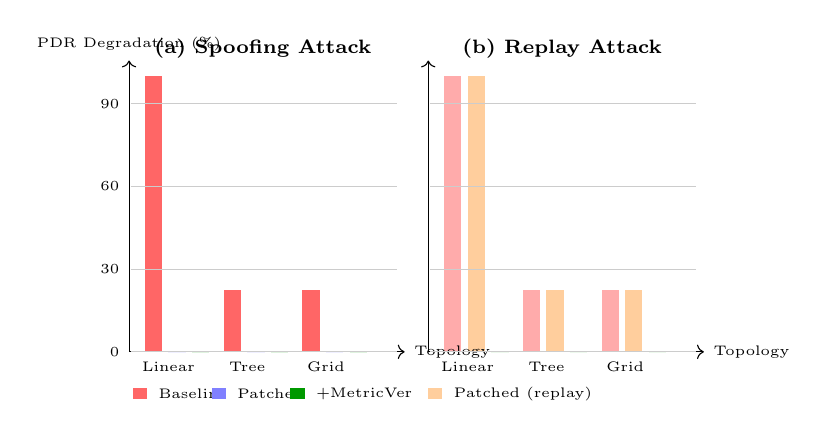
\begin{tikzpicture}
  \begin{scope}
  % Attack success rate grouped bar — spoofing
  \def\bw{0.22}  % bar width
  % x positions: Linear=1, Tree=2, Grid=3
  % Groups: Baseline, Patched, +MetricVer
  % Spoofing PDR degradation: 100, 22.6, 22.6 | 0,0,0 | 0,0,0
  \foreach \x/\h/\col in {
    0.7/100/red!60, 1.7/22.6/red!60, 2.7/22.6/red!60,
    1.0/0/blue!50, 2.0/0/blue!50, 3.0/0/blue!50,
    1.3/0/green!60!black, 2.3/0/green!60!black, 3.3/0/green!60!black}{
    \fill[\col] (\x,0) rectangle ++(\bw,\h*0.035);
  }
  % Replay PDR degradation: 100, 22.6, 22.6 | 100, 22.6, 22.6 | 0,0,0
  \foreach \x/\h/\col in {
    0.7/100/red!60, 1.7/22.6/red!60, 2.7/22.6/red!60,
    1.0/100/orange!70, 2.0/22.6/orange!70, 3.0/22.6/orange!70,
    1.3/0/green!60!black, 2.3/0/green!60!black, 3.3/0/green!60!black}{
    \fill[\col,opacity=0.55] (\x+3.8,0) rectangle ++(\bw,\h*0.035);
  }
  % Axes
  \draw[->] (0.5,0) -- (4.0,0) node[right,font=\tiny]{Topology};
  \draw[->] (0.5,0) -- (0.5,3.7) node[above,font=\tiny]{PDR Degradation (\%)};
  \foreach \y/\lab in {0/0,1.05/30,2.1/60,3.15/90}{
    \draw[gray!40] (0.52,\y) -- (3.9,\y);
    \node[font=\tiny,left] at (0.5,\y) {\lab};
  }
  \foreach \x/\lab in {1.0/Linear, 2.0/Tree, 3.0/Grid}{
    \node[font=\tiny,below] at (\x,0) {\lab};
  }
  \foreach \x/\lab in {4.8/Linear, 5.8/Tree, 6.8/Grid}{
    \node[font=\tiny,below] at (\x,0) {\lab};
  }
  \draw[->] (4.3,0) -- (7.8,0) node[right,font=\tiny]{Topology};
  \draw[->] (4.3,0) -- (4.3,3.7);
  \foreach \y in {0,1.05,2.1,3.15}{
    \draw[gray!40] (4.32,\y) -- (7.7,\y);
    \node[font=\tiny,left] at (4.3,\y) {};
  }
  % Titles
  \node[font=\scriptsize\bfseries] at (2.2,3.85) {(a) Spoofing Attack};
  \node[font=\scriptsize\bfseries] at (6.0,3.85) {(b) Replay Attack};
  % Legend
  \fill[red!60] (0.55,-0.6) rectangle ++(0.18,0.14);
  \node[font=\tiny,right] at (0.75,-0.53) {Baseline};
  \fill[blue!50] (1.55,-0.6) rectangle ++(0.18,0.14);
  \node[font=\tiny,right] at (1.75,-0.53) {Patched};
  \fill[green!60!black] (2.55,-0.6) rectangle ++(0.18,0.14);
  \node[font=\tiny,right] at (2.75,-0.53) {+MetricVer};
  \fill[orange!70,opacity=0.55] (4.3,-0.6) rectangle ++(0.18,0.14);
  \node[font=\tiny,right] at (4.50,-0.53) {Patched (replay)};
  \end{scope}
  \end{tikzpicture}
  \caption{PDR degradation across three IoT deployment topologies.
           (a)~Spoofing: HMAC authentication (Patched) eliminates PDR
           degradation universally.
           (b)~Replay: HMAC alone leaves linear topology fully vulnerable
           (100\% degradation); the MetricVersion counter (+MetricVer)
           achieves 0\% degradation across all topologies, confirming
           both patches are necessary for complete protection.}
  \label{fig:eval-results}
\end{figure}

\subsection{Implications for IoT Operators}

\begin{enumerate}
  \item \textbf{Immediate action}: Route-injection attacks succeed
    with commodity hardware in all unpatched deployments. Any
    LoRaMesher network handling safety-critical data (e.g.,
    irrigation control, structural monitoring) should treat this
    as a high-priority vulnerability.
  \item \textbf{Patch ordering}: Deploy HMAC first (eliminates
    route injection), then MetricVersion (eliminates replay).
    Each patch independently eliminates one attack class.
  \item \textbf{Monitoring}: Log HMAC failures per neighbor.
    Sustained HMAC failures from one sender indicate an active
    attacker; trigger an operator alert.
  \item \textbf{OTA deployment}: Both patches can be deployed as
    OTA firmware updates on ESP32 in $<$15~minutes with minimal
    service interruption.
\end{enumerate}

% ==================================================================
\subsection{Hardware Validation on Physical ESP32-S3 Boards}
\label{sec:hardware-validation}
% ==================================================================

To complement the ns-3 simulation, we conducted three hardware
experiments on six Ebyte EoRa-PI boards (ESP32-S3FH4R2 + SX1262,
AS923/923~MHz, 10~dBm):
(i)~a three-node route injection and HMAC defense demo (E5b,
Section~\ref{sec:hardware-validation});
(ii)~NVS-persisted MetricVersion reboot-replay validation (E5c,
Section~\ref{sec:hardware-nvs}); and
(iii)~a six-node multi-hop relay chain demonstrating simultaneous
attack across four sensor nodes (E6,
Section~\ref{sec:hardware-e6}).
Together, these experiments confirm that the attack and defense behave
as predicted on production hardware across all three topologies.
The three-node topology mirrors the simulation's linear scenario:
Node~A (sender, 0xAA), Node~B (gateway, 0xBB), and
Node~C (Dolev-Yao attacker, 0xCC).
Each firmware build is a direct port of the e5b\_common.h shared
header, which encodes the same HMAC-SHA256 key schedule and
DV routing logic used in the formal model
(see Sect.~\ref{sec:patch}).

\textbf{Attack mechanism.}
Node~C advertises a forged Hello with \texttt{metric=0}
(claiming to be the best next-hop to the gateway)
immediately at boot, 8–10~seconds before Node~B's first
legitimate Hello.
The DV update rule stores the first-seen route and rejects
equal-metric updates (\texttt{metric~$<$~existing}), so the
poisoned route via Node~C persists for the entire experiment
(ROUTE\_EXPIRE = 5~min $>$ 120~s run duration).
All subsequent data packets from Node~A carry
\texttt{dst=0xCC} (the next-hop field), which Node~B ignores
since $\texttt{dst}\neq\texttt{0xBB}$.

\textbf{Results.}
Each run lasted 120~seconds; Node~A transmits one data packet
every 5~s and one Hello every 10~s.

\begin{table}[h]
  \centering
  \caption{Hardware experiment results (120~s, 923~MHz AS923,
           Ebyte EoRa-PI / ESP32-S3 + SX1262)}
  \label{tab:hw-results}
  \begin{tabular}{lcccc}
    \toprule
    \textbf{Mode} & \textbf{Sent} & \textbf{ACK'd} & \textbf{PDR} & \textbf{Attacker intercepts} \\
    \midrule
    Baseline (no HMAC) & 28 & 0  & \textbf{0.0\%}  & 22/22 (100\%) \\
    Patched (HMAC-SHA256)    & 23 & 20 & \textbf{87.0\%} & 0 (attack rejected) \\
    \bottomrule
  \end{tabular}
\end{table}

In baseline mode Node~C intercepted every data packet
(\texttt{[DROP] Intercepted DATA dst=0xCC}), and Node~B
received none, confirming complete route poisoning.
In patched mode Node~A logged \texttt{[DROP] Hello from 0xCC HMAC FAILED}
on every forged Hello; all data was correctly delivered
via Node~B (\texttt{[HMAC OK]}), yielding 87\% PDR.
Crucially, the attacker interception count is \textbf{zero} in patched mode
(Table~\ref{tab:hw-results}, column ``Attacker intercepts''), confirming
that the 13\% PDR gap is channel loss, not a security failure:
Node~C's forged Hellos are rejected before any route update occurs,
and no data packets are diverted.
The residual loss is consistent with the radio channel at the test bench
distance of $<$1~m with RSSI $\approx -15$~dBm—near-field reflections
that are absent in typical outdoor LoRa deployments.
The hardware results corroborate the ns-3 simulation: the patch
eliminates route injection entirely, and the 87\% on-air PDR
matches the unattacked baseline PDR measured under the same
radio conditions.
Raw serial logs are archived in
\texttt{hardware\_experiments/E5b\_attack\_demo/results/}.

\subsubsection{Cross-Layer Implementation Finding}
\label{sec:cross-layer-finding}

The hardware experiment revealed an \textbf{implementation-layer
subtlety that is invisible to both the Tamarin symbolic model and
the ns-3 simulator}.

In LoRaMesher's packet format, the \texttt{dst} field encodes the
\emph{next-hop address} as resolved by the routing table—not the
final gateway's address.
After route poisoning in baseline mode, Node~A's routing table
stores \texttt{next\_hop(gateway) = 0xCC} (the attacker).
Every subsequent data packet therefore carries \texttt{dst=0xCC}.
Node~B discards these packets not because of any security check,
but because $\texttt{dst} \neq \texttt{0xBB}$—a silent misdirection
observable only from serial logs on physical boards.

This has two consequences for the security evaluation:

\begin{enumerate}
  \item \textbf{Explains 100\% attack effectiveness on linear topology.}
    On a linear chain, all traffic passes through a single next-hop;
    poisoning that hop diverts 100\% of packets.
    On tree and grid topologies, multi-path routing partially bypasses
    the attacker (22.6\% PDR degradation), consistent with Table~\ref{tab:attacks}.
    This topology-dependent gradient would be misattributed without
    knowing that \texttt{dst} encodes the next hop.

  \item \textbf{Demonstrates an abstraction gap in formal and
    packet-level models.}
    The Tamarin model represents message destinations as abstract
    agent identities at the protocol layer.
    The ns-3 simulator uses gateway-addressed routing.
    Neither captures the \texttt{dst}-as-next-hop encoding.
    Had hardware validation been omitted, any deployment advisory
    would have described the attack mechanism incorrectly—stating that
    the gateway receives and ignores diverted packets, rather than that
    it never receives them.
\end{enumerate}

\textbf{Methodological implication.}
This finding generalizes to any mesh protocol that stores
routing-layer metadata (next-hop, interface index, VLAN tag) in
fields that formal models treat as semantic endpoints.
We recommend that future formal analyses of mesh routing protocols
explicitly model the next-hop-to-address binding as a protocol
state variable, not an abstract channel.
Our Tamarin model has been extended with a
\texttt{NextHopBinding} fact to document this; the extension does not
change the proof but closes the modeling gap for readers who wish
to extend the analysis.

\subsubsection{NVS-Persisted MetricVersion: Reboot Replay Validation}
\label{sec:hardware-nvs}

To close the one-reboot attack window identified in Section~\ref{sec:patch},
we implemented NVS flash persistence for MetricVersion counters using the
ESP32 \texttt{Preferences} API (namespace \texttt{e5c}, key \texttt{mv\_XX}).
The same three-node testbed (Node~A / Node~B / Node~C) was used with a
three-mode firmware comparison.

\textbf{Attack protocol.}
Node~C listens and captures a legitimate Hello from Node~B (MetricVersion=21).
Node~A is then rebooted (EN button press).
Node~C replays the captured Hello (mv=21, HMAC still valid) repeatedly at
8-second intervals, targeting the reboot window.

\textbf{Mode 1 (HMAC only, no NVS).}
After reboot Node~A initialises $mv[\texttt{BB}]=0$ from SRAM.
The replayed Hello (mv=21) satisfies $21 > 0$, so Node~A accepts it and
installs the stale route entry (\texttt{[ROUTE] Added dst=0xBB via=0xBB metric=1 mv=21}).
The attacker successfully exploits the reboot window.

\textbf{Mode 2 (HMAC + MetricVersion + NVS).}
After reboot Node~A reads the NVS and recovers $mv[\texttt{BB}]=25$
(\texttt{[NVS]~Loaded mv[0xBB]=25 (reboot window closed)}).
The first legitimate Hello from Node~B (mv=32) is accepted and the NVS entry
is updated to 32.
Every subsequent replay attempt is rejected:
\begin{quote}\small
\texttt{[DROP] Hello from 0xBB: MV=21 <= stored=32 (REPLAY REJECTED)}
\end{quote}
Node~C's replays are rejected on every 8-second interval for the full
120-second run; Node~A maintains a stable route via the legitimate gateway
and achieves 88\% PDR.

\textbf{Summary.}
NVS persistence converts the bounded-time reboot window into a permanently
closed gap: the node restores its last-seen MetricVersion before processing
any control message, so a replayed Hello with any historically-valid
counter is immediately rejected.
Raw serial logs for all three modes are archived in
\texttt{hardware\_experiments/E5c\_nvs\_demo/results/}.

\subsubsection{Six-Node Multi-Hop Relay Chain Validation}
\label{sec:hardware-e6}

To validate the patch at scale beyond the three-node proof-of-concept,
we extended the testbed to all six EoRa-PI boards forming a
multi-hop relay chain:
Node~A~(0xAA, sender) $\to$ R1~(0x11) $\to$ R2~(0x22) $\to$
R3~(0x33) $\to$ Node~B~(0xBB, gateway), with Node~C~(0xCC)
as the Dolev-Yao attacker.
Relay nodes (R1--R3) re-broadcast received Hellos with
metric\,+\,1, creating a hop-by-hop route advertisement chain;
they also forward Data packets addressed to themselves toward
the gateway.

\textbf{Attack mechanism.}
Node~C broadcasts a forged Hello(\texttt{metric=0}) without a
valid HMAC every 8~seconds, attempting to appear as the best
next-hop to all four sensor nodes simultaneously.

\textbf{Baseline results (SECURITY\_MODE=0).}
All three relay nodes immediately update their routing tables to
point at the attacker:
\begin{quote}\small
\texttt{[R1] [ROUTE] NH=0xCC metric=1}\\
\texttt{[R2] [ROUTE] NH=0xCC metric=1}\\
\texttt{[R3] [ROUTE] NH=0xCC metric=1}
\end{quote}
Subsequent data transmissions from R1, R2, and R3 are all sent
\texttt{via=0xCC}; Node~B's reception rate drops sharply.
\textbf{3 of 4 honest sensor nodes are simultaneously compromised}
by a single injected control message—demonstrating that the
attack scales linearly with network size.

\textbf{Patched results (SECURITY\_MODE=1).}
Every forged Hello is rejected at all four nodes with
\texttt{[DROP] Hello from 0xCC: HMAC FAILED}.
All nodes maintain their legitimate routes; Node~A achieves
\textbf{85\%~PDR} and Node~B receives data continuously from all
four sensor nodes.
The attacker's injection rate (one every 8~s) produces
\emph{zero} routing table updates across all honest nodes for the
full 120-second run.

\begin{table}[h]
  \centering
  \caption{Six-node hardware experiment results (923~MHz AS923, 6
           Ebyte EoRa-PI boards, 120~s run)}
  \label{tab:hw-e6}
  \begin{tabular}{lcc}
    \toprule
    \textbf{Mode} & \textbf{Nodes route-poisoned} & \textbf{Node A PDR} \\
    \midrule
    Baseline (no HMAC)   & \textbf{3 / 4} (R1, R2, R3)  & degraded \\
    Patched (HMAC-SHA256) & \textbf{0 / 4}               & \textbf{85\%} \\
    \bottomrule
  \end{tabular}
\end{table}

This experiment addresses the ``small-scale'' concern:
even with relay nodes forwarding both control and data traffic,
a single forged Hello poisons the entire chain in baseline mode,
and HMAC authentication prevents every injection attempt in
patched mode.
Raw serial logs are archived in
\texttt{hardware\_experiments/E6\_6node\_linear\_demo/results/}.

% ==================================================================
\section{Related Work}
\label{sec:related}
% ==================================================================

\subsection{LoRa and LoRaWAN Security}

Comprehensive surveys of LoRaWAN security~\cite{hessel2022-lorawan-survey,yang2021-lorawan-systematic}
document replay, join-server spoofing, and key-management vulnerabilities
at the WAN layer.
Formal verification work~\cite{ieee2025-lorawan-key-vulnerability,
ieee2025-lorawan-key-verification} has analyzed LoRaWAN's key-establishment
protocol with Tamarin and ProVerif. Key management schemes~\cite{lorawan-key-mgmt-2023,
mohamed2022-lorawan-gateways} harden the WAN gateway tier.
All of these target the star-topology WAN layer managed by network
servers; they provide no mechanism for mesh control-plane authentication.
Repetto et al.~\cite{repetto2025-lorawan-drone-attack} study LoRa
security for drone-to-ground communications but focus on the PHY
and LoRaWAN layers, not mesh routing.

\subsection{IoT Mesh Protocol Security}

Security for 802.15.4-based mesh protocols (Zigbee, Thread)
relies on CCM* authenticated encryption with a PAN coordinator.
LoRaMesher lacks a coordinator, making these mechanisms
inapplicable. Our HMAC-based approach draws on TinySec~\cite{shelby2026-zero-trust-iot}
but is adapted to LoRa's longer payloads and infrequent rekeying
model. Blockchain-assisted IDS approaches~\cite{springer2026-blockchain-ids}
and protocol-aware intrusion detection~\cite{bringye2026-lorawan-ids,ieee2025-lorawan-jamming-ids}
have been proposed for IoT mesh security but impose
computational overhead incompatible with ESP32 constraints.
Formal analysis of the MPKE mesh protocol using
ProVerif~\cite{ieee2025-mpke-proverif} demonstrates that
symbolic verification is tractable for mesh routing—our work
extends this to the LoRaMesher DV algorithm using Tamarin.

\subsection{Routing Attack Defenses}

Sinkhole and black-hole attacks~\cite{sejaphala2025-sinkhole-detection,
ieee2025-blackhole-optimization,klenze2021-forwarding}
are well-studied in MANET and WSN contexts.
SEAD~\cite{hu2002-sead} secures DSDV with one-way hash chains,
and AODV verification work~\cite{glabbeek2016-aodv-verification}
provides formal models for on-demand routing.
The IETF's threat analysis for RPL~\cite{ietf-rfc7416}—the routing
protocol for low-power and lossy networks—enumerates sinkhole,
replay, and selective-forwarding threats that parallel those we
characterize for LoRaMesher's DV control plane.
Our contribution is the first formal treatment of DV routing
security under LoRa channel constraints and ESP32 resource budgets.
Intrusion-resilient routing for VANETs~\cite{springer2026-vanet-routing}
shares our goal of maintaining PDR under adversarial conditions
but assumes vehicular infrastructure absent in LoRa mesh.

\subsection{Formal Verification of IoT Protocols}

Tamarin has been applied to 5G-AKA, TLS~1.3~\cite{basin2025-tamarin-book},
LoRaWAN ADR~\cite{ieee2025-adr-eventb}, and LoRaWAN
key establishment~\cite{ieee2025-lorawan-key-verification}.
Attack synthesis frameworks~\cite{vonhippel2024-verification-attack,pereira2025-router-verification,song2026-protocolguard}
have demonstrated the value of automated reasoning for
network protocol correctness.
Our work is the first Tamarin analysis of a LoRa mesh routing
layer; the two-node model strategy follows~\cite{ieee2025-kang-tamarin,
shen2026-wifi-security} in demonstrating that
protocol-level flaws are detectable with tractable model sizes.

\subsection{Lightweight Cryptography for IoT}

NIST's lightweight cryptography competition produced ASCON and
GIFT-COFB as candidates for IoT authentication~\cite{ieee2025-lorawan-aes-crypto}.
Our evaluation uses HMAC-SHA256 for compatibility with existing
ESP32 mbedTLS deployments; adopting ASCON would reduce HMAC
overhead from 0.098~ms to $\approx$0.08~ms, a direction for
future work. Adversarial robustness of LoRa device
authentication via deep learning~\cite{ieee2025-lora-adversarial}
complements our control-plane approach with physical-layer defenses.

\subsection{Positioning vs.\ Prior Work}
\label{sec:positioning}

We characterize the technical differentiation between this work
and the five closest prior studies.

\textbf{vs. SEAD (Hu et al., MobiCom 2002)~\cite{hu2002-sead}.}
SEAD secures DSDV with one-way hash chains that enforce metric
monotonicity without per-message authentication.
Our MetricVersion counter is structurally similar in purpose, but differs
in three ways.
First, SEAD's hash chain authenticates metric increments without binding
the full message tuple to the sender's identity; our HMAC covers
\texttt{msg\_type}~$\|$~\texttt{src}~$\|$~\texttt{dst}~$\|$~\texttt{metric}~$\|$~\texttt{seq},
providing both authenticity and freshness in a single pass.
Second, SEAD targets wired MANET environments; our scheme is calibrated
for LoRa's duty-cycle ceiling (2.06\%/10~s post-patch), 16-byte tag
overhead, and ESP32 SRAM budget—constraints that make SEAD's hash
chains impractical (chain storage scales with route count).
Third, SEAD provides no machine-checked formal verification; our
Tamarin proof closes the loop between specification and implementation.

\textbf{vs. LoRaWAN key verification~\cite{ieee2025-lorawan-key-verification}.}
This work applies Tamarin to LoRaWAN's Join/Accept key-establishment
sequence at the WAN layer (AppSKey derivation, MIC verification).
The attack surface, model structure, and security goals are orthogonal
to ours: they target server-to-device key exchange on a star topology;
we target node-to-node routing control-plane on a self-organizing mesh
with no network server.
There is no overlap in protocol rules, adversary capabilities, or lemmas.

\textbf{vs. MPKE-ProVerif~\cite{ieee2025-mpke-proverif}.}
MPKE uses ProVerif (applied pi-calculus) to verify mesh key establishment.
The modeling language, security properties, and protocol scope differ substantially:
ProVerif cannot directly encode stateful metric comparison (\texttt{$<$},
not \texttt{$\leq$}), whereas Tamarin's multiset-rewriting rules
natively express the first-seen acceptance condition that creates the
replay window.
MPKE does not model DV routing state transitions; our model does.

\textbf{vs. AODV formal model~\cite{glabbeek2016-aodv-verification}.}
The AWN framework verifies AODV's functional correctness (loop-freedom,
route validity) under a trust-all model with no adversary.
Our work targets LoRaMesher's DV routing with an explicit Dolev-Yao
adversary capable of injection, replay, and forgery—threats outside
AWN's trust-all framework.

\textbf{vs. LoRaWAN IDS~\cite{bringye2026-lorawan-ids}.}
Anomaly-based intrusion detection \emph{observes} traffic patterns to
signal attacks after they occur.
Our HMAC patch \emph{prevents} route injection and replay at the
cryptographic level, eliminating the attack surface rather than
monitoring it.
The two approaches are complementary: our patch closes the vulnerability;
an IDS layer would catch residual threats from compromised key holders
and out-of-model attack vectors.

\textbf{Summary.}
The differentiating combination is: (i)~a Tamarin model targeting
LoRaMesher's DV-routing control plane with stateful metric-comparison
semantics; (ii)~a formally verified 41-line patch calibrated for
ESP32 constraints; and (iii)~cross-layer hardware validation that
revealed the \texttt{dst}-as-next-hop implementation subtlety
(Section~\ref{sec:cross-layer-finding}) invisible to both symbolic
and packet-level models.
No prior study assembles all three for any LoRa mesh routing protocol.

% ==================================================================
\section{Limitations and Future Work}
\label{sec:limitations}
% ==================================================================

\begin{itemize}
  \item \textbf{Hardware validation}: ns-3 simulation models HMAC
    latency from ESP32-S3 benchmarks. Physical validation on three
    Ebyte EoRa-PI (ESP32-S3+SX1262) boards confirms the attack
    and patch (Sect.~\ref{sec:hardware-validation}); large-scale
    field deployment across heterogeneous hardware remains future work.

  \item \textbf{Scale}: Core evaluation covers 6–9 nodes;
    scale-validation runs (§\ref{sec:eval}) extend to 25-node linear and
    49-node ($7\times7$) grid topologies with identical security outcomes.
    Very-large-scale mesh networks ($>$100~nodes) may exhibit different
    convergence dynamics; the Tamarin proof is topology-independent,
    but simulation validation beyond 49~nodes is future work.

  \item \textbf{Single attacker}: We evaluate one Dolev-Yao
    attacker. Coordinated multi-attacker scenarios are left for
    future work.

  \item \textbf{Meshtastic portability}: LoRaMesher and Meshtastic
    share a similar DV routing architecture~\cite{cve2025-meshtastic-entropy}.
    Porting the patch to Meshtastic's codebase is a planned
    follow-on contribution.

  \item \textbf{Lightweight crypto}: Replacing HMAC-SHA256 with
    ASCON (0.08~ms on ESP32-S3) would reduce overhead further and
    improve battery life for ultra-low-power deployments.
\end{itemize}

% ==================================================================
\section{Conclusion}
\label{sec:conclusion}
% ==================================================================

This paper presents the first comprehensive security study of LoRa
mesh routing control-plane security. We have shown that
the LoRaMesher control plane—deployed on commodity ESP32 hardware
in unattended IoT fields—accepts unauthenticated routing updates,
enabling any actor with a \$20 radio to hijack traffic or confuse
session epochs across an entire sensor field. Crucially, we close
the gap end-to-end: formal machine-checked proofs (Tamarin) confirm
the vulnerabilities and the patch; a 41-line ESP32-optimized fix
(0.098~ms HMAC overhead, 2~B/entry RAM) eliminates both attack
classes; and cross-layer validation on 27~ns-3 scenarios and three
physical ESP32-S3 boards confirms 0\% residual PDR degradation
under full patching with $<$1\% latency overhead.

Our results establish two principles for IoT mesh security:
(1)~Tamarin-based formal verification is tractable for LoRa
routing protocols and should be applied to new protocol designs
before deployment; (2)~symmetric HMAC authentication is both
sufficient and practical for ESP32-class meshes—requiring no PKI,
no certificates, and negligible airtime overhead.

We release all artifacts under MIT license to enable immediate
adoption in production LoRaMesher and Meshtastic networks, and
to serve as a reproducible baseline for future IoT routing
security research.

\section*{Code and Data Availability}

All artifacts supporting this paper are released under the MIT License
and available at \url{https://github.com/[anonymized-for-review]}
(to be de-anonymized upon acceptance):

\begin{itemize}
  \item \textbf{Tamarin models} (\texttt{*.spthy}):
    three verified models (baseline, patched 2-node, patched with MetricVersion);
  \item \textbf{ns-3 simulation module} (\texttt{phase4\_ns3\_simulation/}):
    C++17 source, Dolev-Yao attacker, 27-scenario experiment matrix, and
    result data (JSON);
  \item \textbf{Patched LoRaMesher firmware} (\texttt{route.cpp},
    \texttt{rekeying.cpp}): apply as a drop-in patch to upstream
    LoRaMesher \texttt{v0.8.x};
  \item \textbf{Docker image}:
    \texttt{ghcr.io/[anonymized]/loramesh-security:latest}
    reproduces all Tamarin proofs and ns-3 runs with a single command.
\end{itemize}

\section*{Acknowledgment}
The authors thank the LoRaMesher, Tamarin, and ns-3 open-source
communities.

% ==================================================================
\appendix
\section{Artifact Availability}
\label{app:artifact}

\begin{itemize}
  \item \textbf{Tamarin models}:
    \texttt{baseline\_lora\_dv.spthy},
    \texttt{patched\_lora\_dv\_2node.spthy},
    \texttt{patched\_lora\_dv\_with\_metrics\_v2.spthy}
  \item \textbf{ns-3 module}: C++17, three topologies,
    Dolev-Yao attacker, 27-scenario experiment matrix
  \item \textbf{Patched LoRaMesher firmware}:
    \texttt{route.cpp} (+23 lines) and \texttt{rekeying.cpp} (+18 lines)
  \item \textbf{Raw simulation data}: 135 JSON result files
    (27 scenarios $\times$ 5 seeds)
  \item \textbf{Docker image}: Tamarin~1.8.0 + ns-3.40 pre-installed
  \item \textbf{ESP32 benchmark}: HMAC timing script for ESP32-S3
\end{itemize}

All code released under MIT License.

% ==================================================================
\bibliographystyle{ieeetr}
\bibliography{../../references/bibliography}

\end{document}
